\documentclass{article}
\usepackage{graphicx} % Required for inserting images
\usepackage{amsmath}

\title{Lab 1 Report}
\author{Moaaz Mostafa Ibrahim \hspace{20pt} 2400862}
\date{}

\begin{document}
\maketitle
\section*{Question 1}
"A sensor produces a voltage output ranging from -2.4 V to -1.1 V. To interface with 
an analog-to-digital converter (ADC), this voltage range must be shifted and scaled to span 0 to 
2.5 V. Design the necessary signal conditioning circuit to achieve this transformation and simulate 
the circuit in SIMULINK to verify its performance."\\
\noindent
\\
We must first shift by 2.4 V using a summing amplifier, then use an inverting amplifier with a gain of $\frac{25}{13}$ to scale the voltage. We can use a sinusoidal voltage source and a scope to verify the performance of the circuit.

\begin{figure}[h]
    \centering
    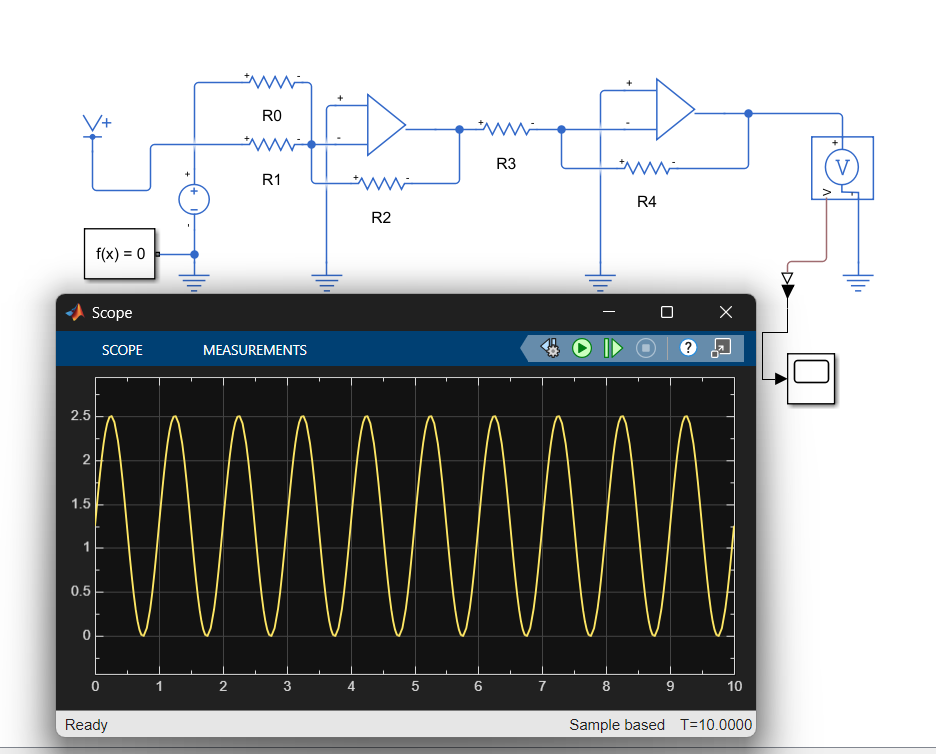
\includegraphics[width=0.95\linewidth]{Media/Q1.png}
\end{figure}
\noindent
The circuit was designed such that $R_0 = R_1 = R_2$ and $R_4 = \frac{25}{13} R_3$

\section*{Question 2}
"A sensor generates a voltage output ranging from 0 to 1 V. Design a voltage-to-current 
converter that converts this range into a corresponding current of 0 to 10 mA. Determine the 
maximum allowable load resistance, given that the operational amplifier saturates at ±10 V. Design 
the necessary signal conditioning circuit to achieve this transformation and simulate the circuit in 
SIMULINK to verify its performance."\\
\noindent
\\
To generate a current of 0 to 10 mA, we must first invert the input voltage using an inverting amplifier with two equal resistances before feeding the voltage to the voltage-to-current converter which operates according to these equations.\\

\begin{align}
    &I = -\frac{R_2}{R_1 R_3} V_{in}\\
    &R_1 (R_3 + R_5) = R_2 R_4
\end{align}

\begin{figure}[h]
    \centering
    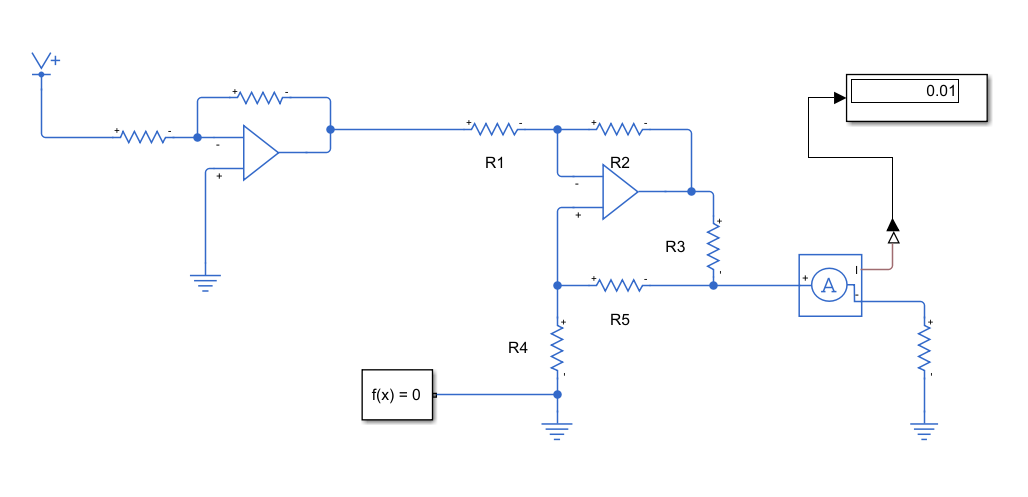
\includegraphics[width=1\linewidth]{Media/Q2.png}
\end{figure}
\noindent
From equation (1), we can assume $R_1 = R_3 = 0.5 k\Omega$ and $R_2 = 2.5 k\Omega$ to get our desired output current. Then using equation (2) we find that $R_5 =5R_4 - 0.5$, so if we let $R_4 = 0.5 k\Omega$ then $R_5 = 2k\Omega$. \footnote{We can also use $R_1 = R_2 = R_4 = 1k\Omega$, $R_3 = 100\Omega$, and $R_5 = 900\Omega$}\\

\noindent
To calculate the maximum load, we use the formula
\begin{align*}
    R_{m} &= \frac{(R_4 + R_5) \left[ \frac{V_{\text{sat}}}{I_{\text{m}}} - R_3 \right]}{R_3 + R_4 + R_5}\\
    R_m &= \frac{(500 + 2000)[\frac{10}{0.01} - 500]}{500+500+2000}\\
    R_m&= \frac{1250}3\Omega \approx 416.667\Omega
\end{align*}

\noindent
Note that if we had used the assumptions $R_1 = R_2 = R_4 = 1k\Omega$, $R_3 = 100\Omega$, and $R_5 = 900\Omega$, we would get $R_m = 855\Omega$.

\end{document}
